\section{Java Message Service}

To handle the producer-consumer problem Java provides a Java Message Oriented Middleware API called the Java Message Service (JMS) API for sending and receiving messages between two or more clients \parencite{jms_wiki}.
JMS being a part of the Java Enterprise Edition (JEE) allows application based on Java EE to create, send, receive and also read messages. It provides the provision for communication between the various components to be loosely coupled, asynchronous and reliable in a distributed application. 

JMS API allows communication that is not just loosely coupled but also the following:

\begin{itemize}
    \item \textbf{Asynchronous:}
          Messages can be delivered to a client as they arrive by a JMS provider. The client need not request messages to receive them.

    \item \textbf{Reliable:}
          JMS API provides different levels of reliability for message delivery. It can be that the message needs to be delivered only once or any other lower reliability level in case an application is not concerned about missing or duplicate messages.

\end{itemize}

\subsection {JMS Elements}
The elements of JMS are described below:

\begin{itemize}
    \item \textbf{JMS Provider:}
          It is an implementation of the JMS interface either as a Java implementation or an adapter to a non-Java implementation. 

    \item \textbf{JMS Client:}
        Any application that produces and/or receives messages.

    \item \textbf{JMS producer:}
        Also referred as publisher. Any JMS client that creates and sends messages. 

    \item \textbf{JMS consumer:}
        Also referred as a subscriber. Any JMS client that is interested in receiving the messages.

    \item \textbf{JMS message:}
        It can be any data that is being transmitted between two or more JMS clients.

    \item \textbf{JMS queue:}
        It is a staging area where the messages that are waiting to read are contained. The message can be read by only one consumer. Unlike its name \textit{queue} suggests, the messages need not received in the same order as they were sent. The JMS queue is only responsible for every message to be processed only once.

    \item \textbf{JMS topic:}
        A logical channel for multiple consumers to receive the same message sent by producers.

    \item \textbf{JMS connection factory:}
        It is an object that encapsulates administrator defined configuration parameters that can be used to create a connection to a provider.

    \item \textbf{JMS destinations:}
        It is an object that represents the target for messages that the client produces or the source of messages that client consumes. The destination can either be a queue or a topic or both.

    \item \textbf{JMS administered objects:}
        The JMS connection factory objects and JMS destination objects are both managed administratively rather than programmatically and hence they are termed as administered objects.

    \item \textbf{JMS sessions:}
        Sessions are a single threaded context that can be used either for producing and consuming messages.
        Entities such as message producer, message consumers and also messages are created using the session object.

\end{itemize}

\subsection {JMS API Architecture}
    \makeatletter
    \setlength{\intextsep}{20pt}
    \makeatother

    \begin{figure}[h!]
    \centering
    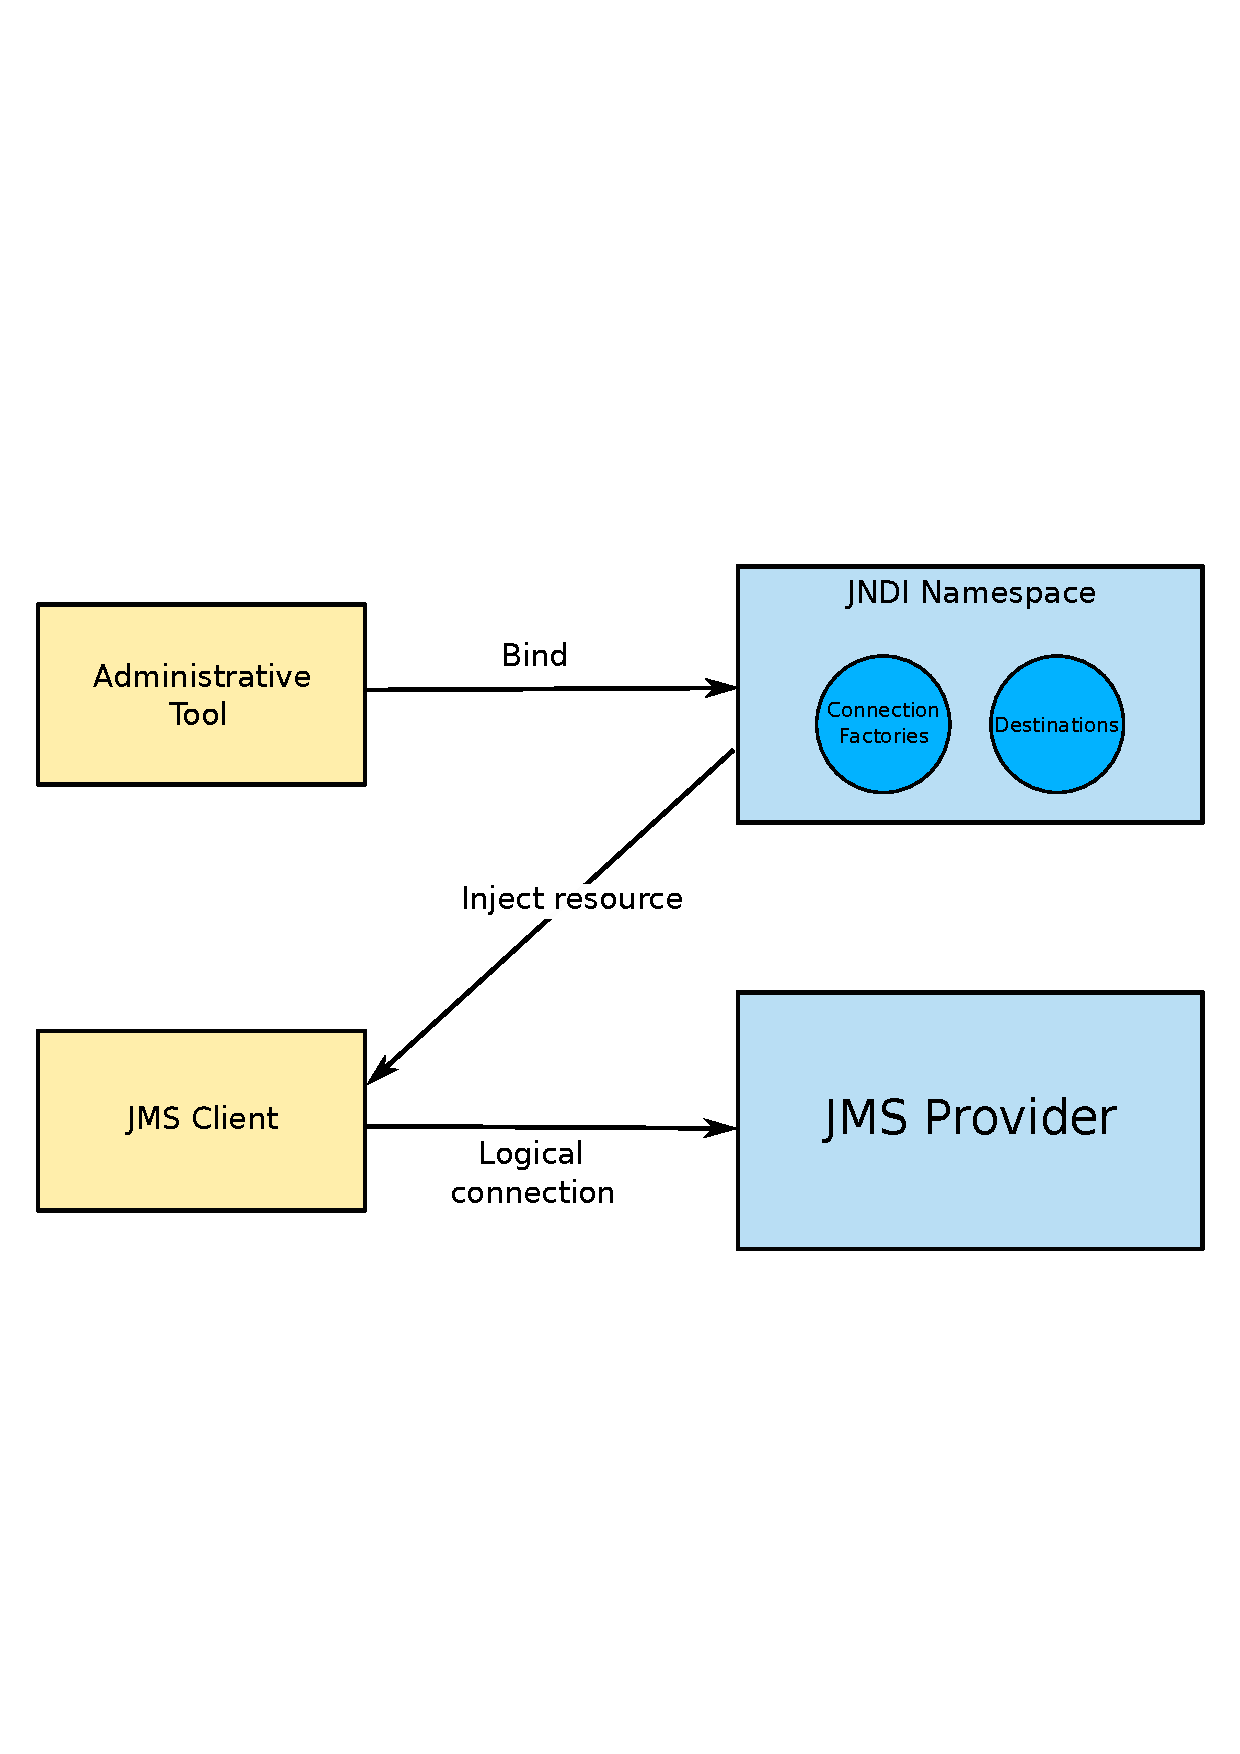
\includegraphics[keepaspectratio, width=.8\textwidth, trim={0 0 0 0},clip]{jms_api.pdf}
    \caption{JMS API Architecture}\label{figures:jms_api}
    \end{figure}

    Figure \ref{figures:jms_api} depicts the way the JMS components interact \parencite{jms_api}. The administrative tools do the binding between the connection factories and destinations into a JNDI namespace.
    The JMS client uses resource injection to access the objects in the namespace and establish a logical connection to the same objects via the JMS provider. 


 \subsection {JMS API Programming Model}

Figure  \ref{figures:jms_api_programming} shows how the basic building blocks of JMS interact in a JMS client application. The connection factory creates the connection object with in turn is used to create a session. As discussed before a session object can be used to create a message, message producer, and message consumer.

    \makeatletter
    \setlength{\intextsep}{20pt}
    \makeatother

    \begin{figure}[h!]
    \centering
    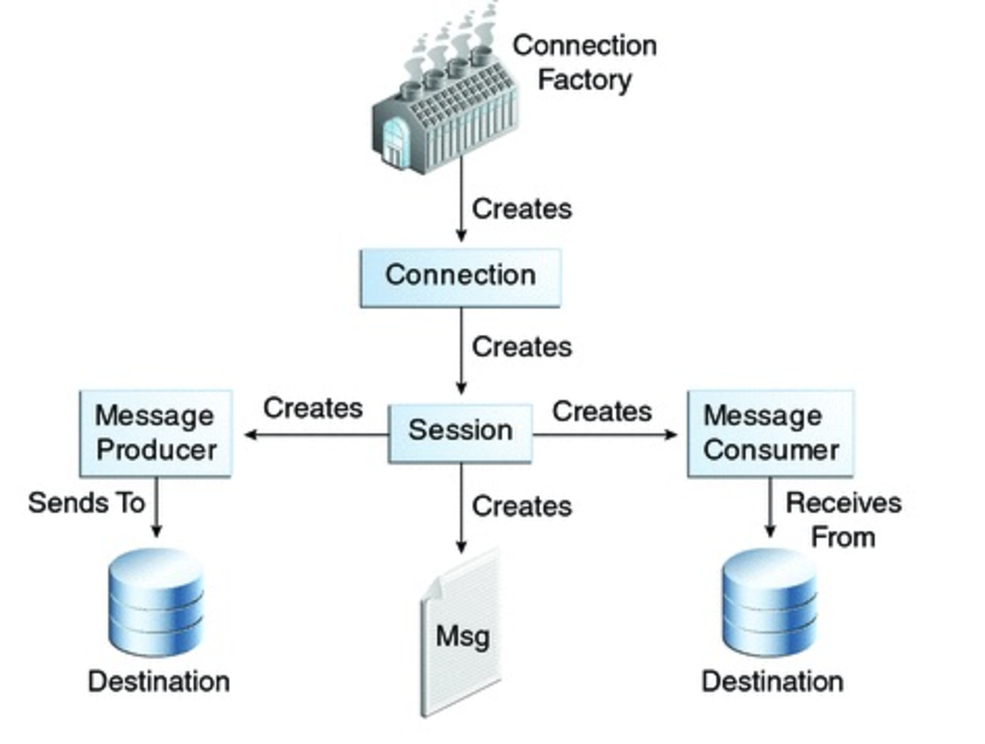
\includegraphics[keepaspectratio, width=.8\textwidth, trim={0 0 0 0},clip]{jms_api_programming.pdf}
    \caption{JMS API Programming Model}\label{figures:jms_api_programming}
    \end{figure}

The JMS programming API minimizes the concepts that are required to build messaging systems at the same time facilitates sufficient features to even maintain sophisticated messaging systems.

